\documentclass[10pt,twocolumn,letterpaper]{article}

\usepackage{cvpr}
\usepackage{times}
\usepackage{epsfig}
\usepackage{graphicx}
\usepackage{amsmath}
\usepackage{amssymb}
\usepackage[lined,algonl,boxed]{algorithm2e}
\usepackage{algorithmic}

% Include other packages here, before hyperref.

% If you comment hyperref and then uncomment it, you should delete
% egpaper.aux before re-running latex.  (Or just hit 'q' on the first latex
% run, let it finish, and you should be clear).
\usepackage[pagebackref=false,breaklinks=true,letterpaper=true,colorlinks,bookmarks=false]{hyperref}


%\cvprfinalcopy % *** Uncomment this line for the final submission

\def\cvprPaperID{1333} % *** Enter the CVPR Paper ID here
\def\httilde{\mbox{\tt\raisebox{-.5ex}{\symbol{126}}}}

% Pages are numbered in submission mode, and unnumbered in camera-ready
\ifcvprfinal\pagestyle{empty}\fi

\begin{document}

%%%%%%%%% TITLE
\title{Domain-Unifying Embedding}
%\author{ Ruonan Li and Todd Zickler\\
%Harvard School of Engineering and Applied Science\\
%{\tt\small \{ruonanli,zickler\}@seas.harvard.edu}
%}

\maketitle
% \thispagestyle{empty}

\begin{abstract}
We propose \textit{Domain Unifying Embedding}, together with its kernelized version, as a consolidated framework for domain adaptation and cross-domain recognition. Our approach embeds samples from one or more source domains and a target domain into a single latent shared domain, with the embedding represented by a linear or kernel transformation. In addition to allowing an arbitrary number of source domains, the approach allows domains to be heterogeneous in the sense of having different dimensions. It also allows simultaneously exploiting a variety of types of semi-supervision, including target samples with explicit class labels when available, and instances for which corresponding, but unlabeled, samples are available in two or more domains.
\end{abstract}

\section{Introduction}

\begin{figure}[t]
\begin{center}
%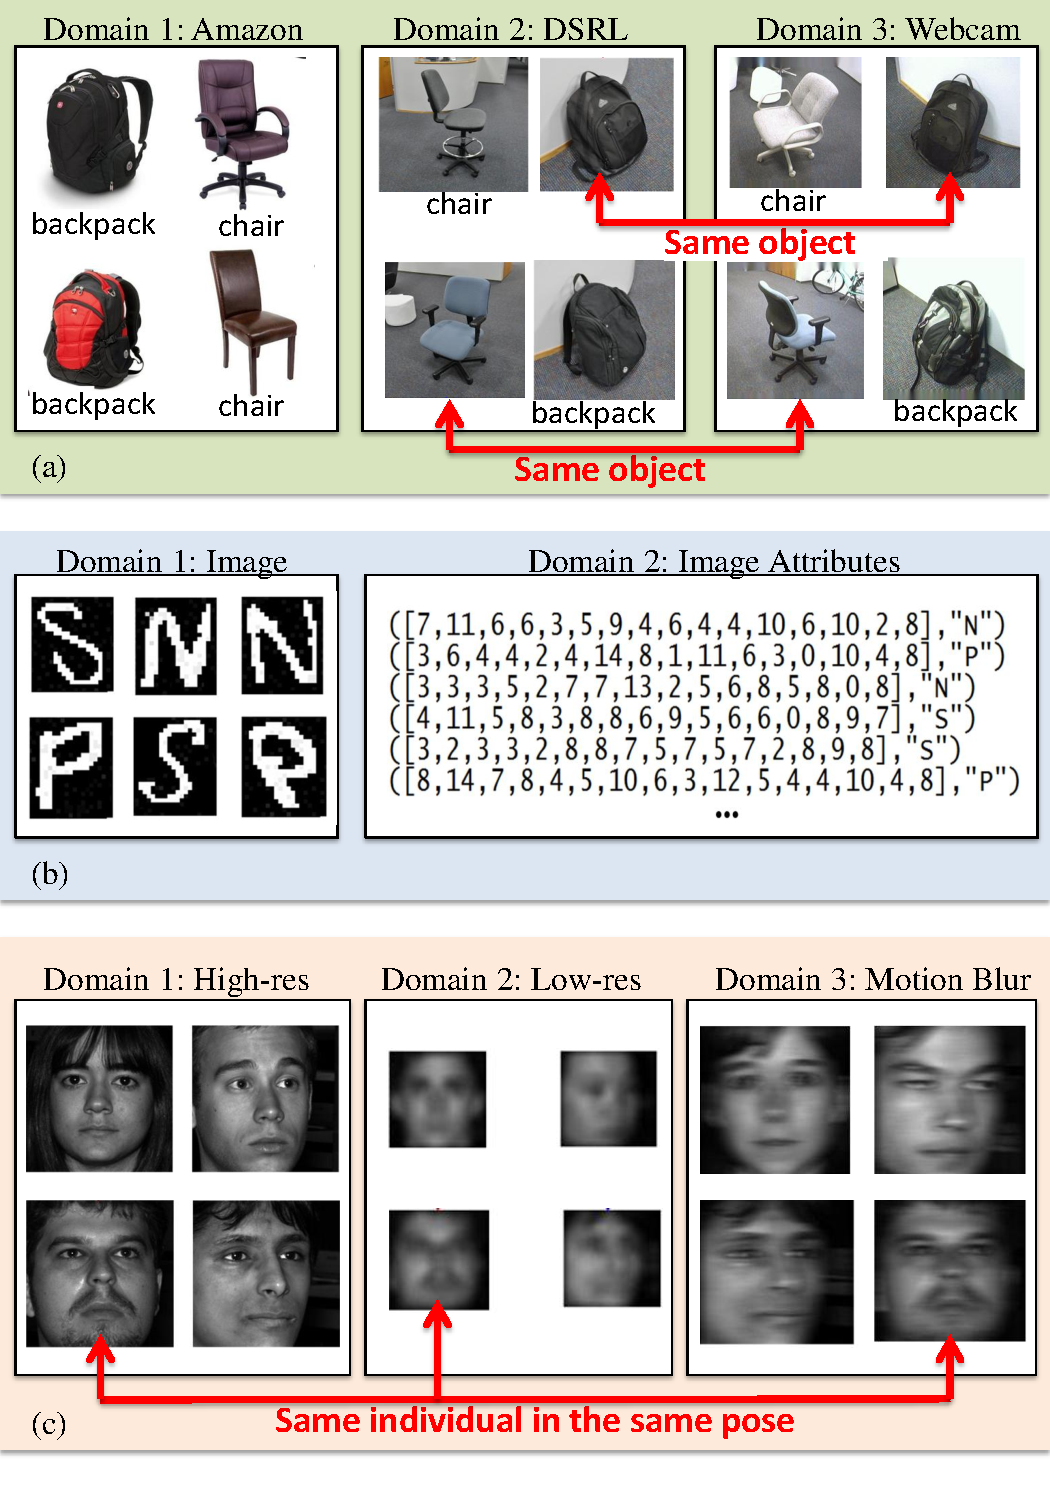
\includegraphics[width=\columnwidth]{due-fig.png}
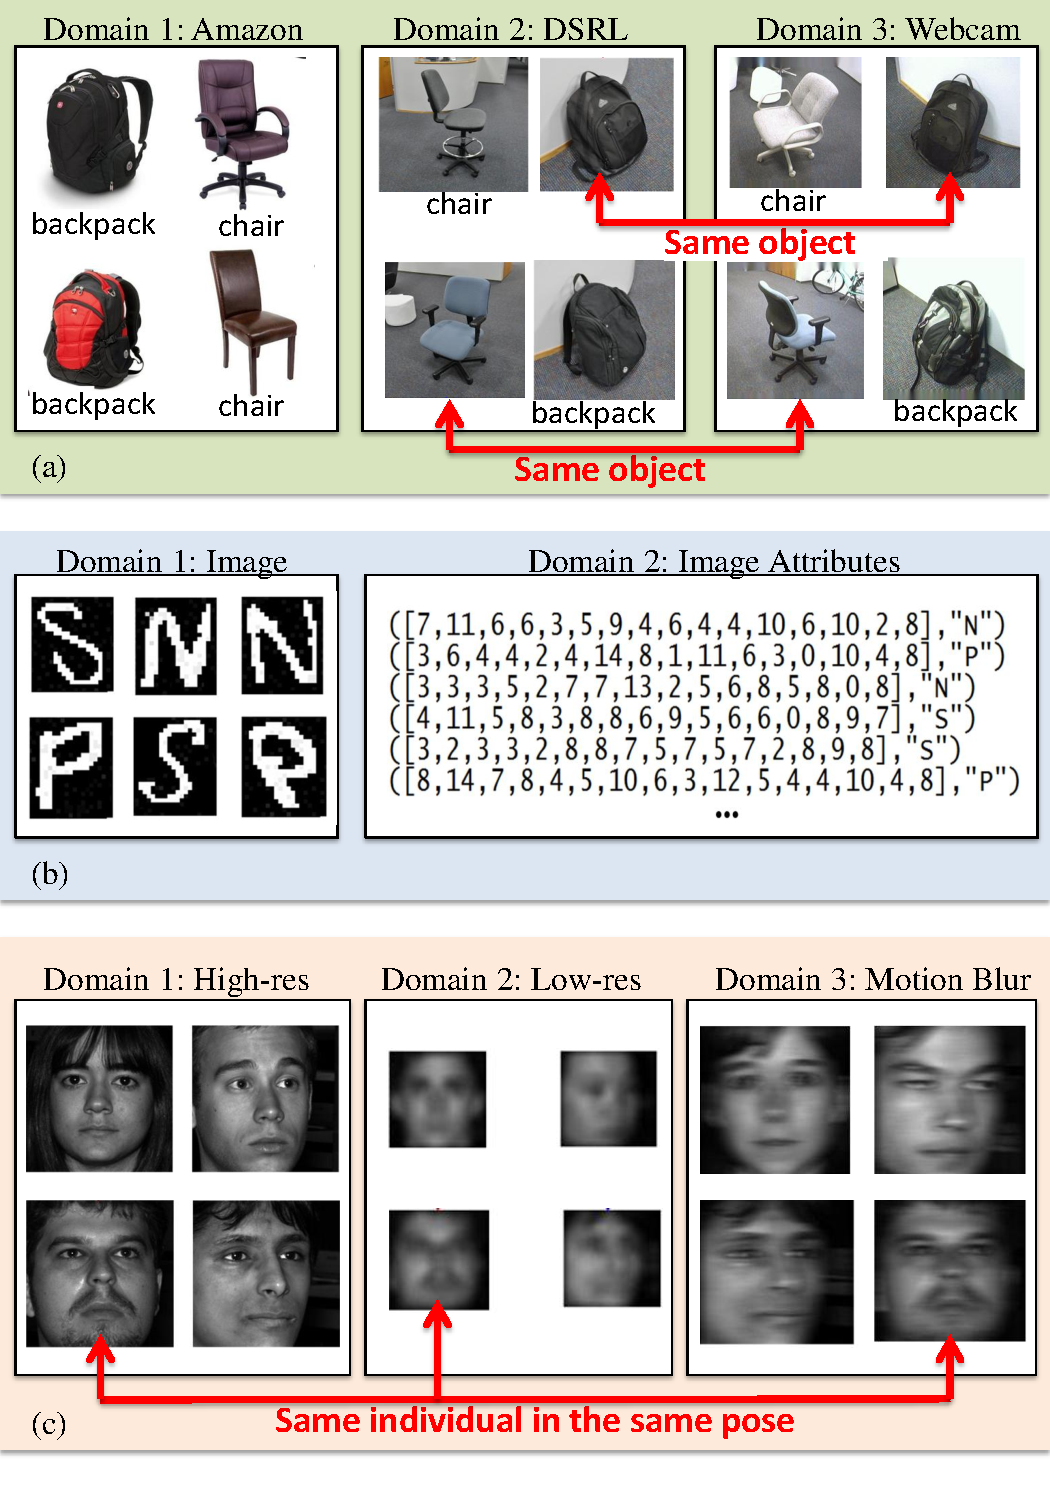
\includegraphics[width=\columnwidth]{due-fig.pdf}
\end{center}
\vspace{-0.2in}
\caption{Our Domain-Unifying Embedding approach can seamlessly handle all of the following scenarios: more than two domains (a,c); heterogeneous features (b); both label and correspondence (red arrows) constraints (a,c). See Section~\ref{exp} for more details on these datasets.}
\label{illu}
\end{figure}


In pattern classification, the distribution of samples to be classified is often different from that available for training. This is the situation, for example, when sufficient numbers of labels are too expensive or time-consuming to obtain for the dataset to be classified but are abundantly available for a different related dataset. Regardless of the cause, any distributional change that occurs after learning can degrade classification performance, and domain adaptation (or domain-transfer learning) \cite{Daume:DA, Ben-David:analysis,Blitzer:DA,Ben-David:DA, Pan:survey} aims at lessening this degradation.

A common domain adaptation problem involves a \textit{source} domain, where samples are well-annotated with class labels and a discriminative classifier can be trained, and a \textit{target} domain, where very few annotations are available. The domains are often assumed to be \emph{homogeneous} in the sense of having the same underlying dimension. The goal is to leverage the rich label information in the source domain to improve classification performance in the target domain by discovering and modeling the statistical relationship between them. Effective approaches for such adaptation from a single source domain include transferring support vector machines (SVMs) between domains \cite{Daume:simpleSVM,Bruzzone:DASVM,Duan:MKL,Schweikert:SVMsurvey,Bergamo:SVMsurvey}, transforming features between them through linear dimension reduction \cite{Ling:Spectral,Pan:TCA} or similarity learning \cite{Kulis:ML,Saenko:ML}, and creating cross-domain features through subspace interpolation \cite{Gopalan:Grassmann, Gong:Grassmann}. 

This paper considers a generalized domain adaptation problem, one that is broadened in three respects(see Figure~\ref{illu}). First, we consider the case when more than one source domain is available. An example is the problem of recognizing objects in images taken by a smartphone, when available annotations exist in two or more different sources (amazon.com, PASCAL VOC\cite{Everingham10}, etc.). Second, we allow the domains to be heterogeneous, with distinct underlying dimensionalities caused by differences in modality (MRI, CT, X-Ray, etc.), different sensor characteristics (e.g., sensors with different spatial and spectral resolutions), or anything else. Third and finally, we allow a more varied form of semi-supervision: In addition to class labels in the source domains (and perhaps the target domain), we consider the availability of unlabeled instances that are simultaneously observed as samples in two or more domains. For example, we may know that an action is being performed by the same actor and being observed simultaneously by two surveillance cameras from two viewpoints, without knowing what type of action he/she is performing. We refer to such unlabeled samples as \emph{correspondences} among domains, and in many situations they are more available than explicit class labels. Our intention is to use them as another source of useful information about the statistical relationships: 1) between different source domains; and 2) between source and target domains. 

Subsets of these three generalizations have appeared separately. Heterogeneity was considered in \cite{Shi:heterogeneous,Zhu:heterogeneous,Duan:heterogeneous}, and multiple sources are the focus of \cite{Crammer:multi,Mansour:multi-domain,Chattopadhyay:multi-domain,Duan:multi-SVM,Wang:Manifold}. Unlabeled correspondences have been largely ignored in domain adaptation for cross-domain recognition, while they have been studied in canonical correlation analysis (CCA) \cite{CCA} and multi-view learning \cite{Ruping:multi-view,Sindhwani:multi-view,Zhou:multi-view,Christoudias:multi-view,Amini:multi-view,Harel:multi-view}. The main contribution of this paper is a computational model that incorporates all of these generalizations simultaneously. It will become evident that our approach also accommodates completely unsupervised adaptation as considered in \cite{Gopalan:Grassmann, Gong:Grassmann, Shi:Unsupervised}.

We introduce \emph{Domain-Unifying Embedding} as a tool for domain adaptation in the presence of multiple heterogeneous source domains, unlabeled correspondences between domains, and (optionally) a partially labeled target domain. The idea is to compute an optimal linear or kernel embedding that brings heterogeneous features from the target domain and the many source domains to a single common domain of pre-specified dimension. The embedding comes from solving a generalized eigenvalue problem that, analogous to the dimensionality-reducing approach of \cite{graphembedding}, is interpreted as embedding a cross-domain graph with affinities that encode information from class labels and unlabeled correspondences within and between the various domains. These affinities are weighted with adaptive weights that are optimized for the input dataset.

Our approach can be applied without change to conventional domain adaption problems, with performance comparable to the state-of-the art. Its main advantage is in utilizing the maximum available information, thus allowing performance improvements when additional sources are available, when domains are heterogeneous, and when there are unlabeled correspondences between domains.


\section{Domain-Unifying Embedding}



Consider $V$ domains enumerated by $v\in\{1,\ldots,V\}$, with the underlying dimension of the $v$th domain represented by $d_v$, a positive integer. Let us call the first domain ($v=1$) the target domain, even though it receives no special treatment as will become clear. Also consider $N$ entities. The $n$th entity is represented by the tuple $O(n)=\{z_{n}, \mathbf{v}_{n}, \{ \mathbf{y}_{n,v} \}_{v} \}$. The class label $z_n\in\{-1,1,2,\ldots,Z\}$ indicates to which of $Z$ categories the entity belongs, where $z_n=-1$ indicates that the entity is unlabeled. $\mathbf{v}_n$ is a $V\times 1$ binary indicator vector where $\mathbf{v}_n(v)=1$ means that the $n$th entity is observed in the $v$th domain and $\mathbf{v}_n(v)=0$ means otherwise. Finally, for each domain $v$ observing the $n$th entity (\textit{i.e.}, when $\mathbf{v}_n(v)=1$), the tuple includes a $d_v$-dimensional feature vector $\mathbf{y}_{n,v}$.

An entity can be labeled or unlabeled in this model. It can be instantiated in only one domain (and therefore no correspondence among domains exists for this entity), or it can be instantiated in two or more domains (and therefore correspondence exists among domains). The underlying dimensions $d_v$ of the domains can be different. Thus, this representation encompasses all of the generalizations discussed in the introduction.

We seek a linear embedding (dimension reduction) to bring observations in all $V$ domains to a $(V+1)$th $k$-dimensional latent domain where each of the heterogeneous domain-specific features is represented by an $k$-dimensional feature in this unifying latent domain. We formulate this as a graph embedding problem \cite{graphembedding} in the form of a generalized eigen decomposition
\begin{equation}
\label{GED}
\tilde{\mathbf{L}}\mathbf{w}=\tilde{\mathbf{B}}\mathbf{w}\mathbf{\Lambda},
\end{equation}
where $\mathbf{w}=[\mathbf{w}_{1}^{T}, \mathbf{w}_{2}^{T}, \cdots, \mathbf{w}_{V}^{T}]^{T}$ is a $(\sum_{v=1}^{V}d_{v})\times k$ linear transformation in which the the $(d_v\times k)$ sub-matrix $\mathbf{w}_{v}$ is the portion of that embedding that operates on the $v$th domain. Matrices $\tilde{\mathbf{L}}$ and $\tilde{\mathbf{B}}$ are of the form of $\tilde{\mathbf{L}}=\mathbf{X}\mathbf{L}\mathbf{X}^{T}$ and $\tilde{\mathbf{B}}=\mathbf{X}\mathbf{B}\mathbf{X}^{T}$ respectively, with the matrix $\mathbf{X}$ being a block-diagonal matrix, whose $(v,v)$th block is a $d_{v}\times(\sum_{n=1}^{N}\mathbf{v}_{n}(v))$ submatrix  assembling all feature vectors observed in domain $v$ as its columns. Matrices $\mathbf{L}$ and $\mathbf{B}$ are the Laplacian matrices of two graphs which encode all different types of pair-wise relationships (see below) between all of these feature vectors. 


 We denote by $\mathbf{W}$ the affinity matrix corresponding to Laplacian $\mathbf{L}$, and by $\mathbf{U}$ that corresponding to Laplacian $\mathbf{B}$.  Both affinity matrices are symmetric and of size  $\sum_{n=1}^{N}\sum_{v=1}^{V}\mathbf{v}_{n}(v)$. Each of the two graphs is composed of $V$ sub-graphs, with each sub-gragh representing the samples from the same domain. Consequently, the affinity matrix $\mathbf{W}$ (resp. $\mathbf{U}$) is composed of $V\times V$ blocks, among which the block $\mathbf{W}_{i,j}$ (resp. $\mathbf{U}_{i,j}$) encodes the affinity information between samples from domain $i$ and those from domain $j$. Note that $\mathbf{W}_{i,j}$ and $\mathbf{U}_{i,j}$ are both $(\sum_{n=1}^{N}\mathbf{v}_{n}(i))\times(\sum_{n=1}^{N}\mathbf{v}_{n}(j))$ matrices and $\mathbf{W}_{i,j}^{T}=\mathbf{W}_{j,i}$ (resp. $\mathbf{U}_{i,j}^{T}=\mathbf{U}_{j,i}$). The diagonal blocks $\mathbf{W}_{i,i}$ (resp. $\mathbf{U}_{i,i}$) $i=1,2,\cdots,V$ encode the similarities between samples from within domain $i$, and the off-diagonal blocks $\mathbf{W}_{i,j}$ (resp. $\mathbf{U}_{i,j}$) $i,j=1,2,\cdots,V, i\neq j$ encode the similarities between samples from domain $i$ and samples from domain $j$. 

\vspace{5pt}
\noindent\textbf{Intra-Domain Affinity}. Assume entity $n_{1}$ and entity $n_{2}$ are both observed in domain $i$ (\textit{i.e.}, $\mathbf{v}_{n_{1}}(i)=\mathbf{v}_{n_{2}}(i)=1$), and let the $(k_{i},l_{i})$th element of $\mathbf{W}_{i,i}$, $W_{i,i}(k_{i},l_{i})$, to be the affinity between them in domain $i$. We define
\begin{equation}
\label{Wintra}
W_{i,i}(k_{i},l_{i})=\frac{1}{N_{i}^{2}}(c_{1,i}^{2}e^{-\frac{\|\mathbf{y}_{n_{1},i}-\mathbf{y}_{n_{2},i}\|^{2}}{\sigma^{2}}}+c_{2,i}^{2}\delta(z_{n_{1}}=z_{n_{2}})),
\end{equation}
where $N_i\triangleq \sum_{n=1}^{N}\mathbf{v}_{n}(i)$ is the total number of samples shown in the $i$th domain.
Similarly, we define
\begin{equation}
\label{Uintra}
U_{i,i}(k_{i},l_{i})=\frac{1}{N_{i}^{2}}d_{1,i}^{2}\delta(z_{n_{1}}\neq z_{n_{2}}).
\end{equation}
Here the positive coefficients $c$ and $d$ serve as adaptable weights. We will discuss how to learn them shortly.
 
\vspace{5pt}
\noindent\textbf{Inter-Domain Affinity}. Assume entity $n_{1}$ is observed in domain $i$ (\textit{i.e.}, $\mathbf{v}_{n_{1}}(i)=1$) and entity $n_{2}$ is  observed in domain $j$ (\textit{i.e.}, $\mathbf{v}_{n_{2}}(j)=1$), and let the $(k_{i},l_{j})$th element of $\mathbf{W}_{i,j}$, $W_{i,j}(k_{i},l_{j})$, be the affinity between them. We define
\begin{equation}
\label{Winter}
W_{i,j}(k_{i},l_{j})=\frac{1}{N_{i}N_{j}}(c_{3,i}c_{3,j}\delta(n_{1}=n_{2})+c_{2,i}c_{2,j}\delta(z_{n_{1}}=z_{n_{2}})).
\end{equation}
Similarly, we define
\begin{equation}
\label{Uinter}
U_{i,j}(k_{i},l_{j})=\frac{1}{N_{i}N_{j}}(d_{2,i}d_{2,j}\delta(n_{1}\neq n_{2})+d_{1,i}d_{1,j}\delta(z_{n_{1}}\neq z_{n_{2}})).
\end{equation}

\subsection{Intuition}

It is straightforward to prove that if all coefficients $c$ and $d$ are given, by solving (\ref{GED}) for the generalized eigen vectors corresponding to the smallest $k$ eigenvalues, we essentially perform the constrained minimization 
\begin{equation}
\label{rayleigh}
\min_{\mathbf{w}}tr(\mathbf{w}^{T}\tilde{\mathbf{L}}\mathbf{w}), \textup{s.t.}\hspace{3pt}tr(\mathbf{w}^{T}\tilde{\mathbf{B}}\mathbf{w})=\textup{constant},
\end{equation} 
which commonly serves as a substitute solution for minimizing the Rayleigh Quotient $\frac{tr(\mathbf{w}^{T}\tilde{\mathbf{L}}\mathbf{w})}{tr(\mathbf{w}^{T}\tilde{\mathbf{B}}\mathbf{w})}$, where the numerator is
\begin{equation}
tr(\mathbf{w}^{T}\tilde{\mathbf{L}}\mathbf{w})=\sum_{i,j=1}^{V}\sum_{k_{i}=1}^{N_i}\sum_{l_{j}=1}^{N_j}\|\mathbf{w}_{i}^{T}\mathbf{y}_{n_{1},i}-\mathbf{w}_{j}^{T}\mathbf{y}_{n_{2},j}\|^{2}W_{i,j}(k_{i},l_{j}),
\end{equation}
and the denominator is
\begin{equation}
tr(\mathbf{w}^{T}\tilde{\mathbf{B}}\mathbf{w})=\sum_{i,j=1}^{V}\sum_{k_{i}=1}^{N_i}\sum_{l_{j}=1}^{N_j}\|\mathbf{w}_{i}^{T}\mathbf{y}_{n_{1},i}-\mathbf{w}_{j}^{T}\mathbf{y}_{n_{2},j}\|^{2}U_{i,j}(k_{i},l_{j}).
\end{equation}

Since entries $W_{i,j}(k_{i},l_{j})$ and $U_{i,j}(k_{i},l_{j})$  encode the objectives and regularizations we aim to achieve, this solution provides the optimal embedding for a given annotated training set. Specifically, a penalty is incurred for each pair of features projected into the latent domain: For a pair of projected feature vectors arising from the same domain, (\ref{Wintra}) incurs a penalty for those close to each other and from the same category, and (\ref{Uintra}) incurs a penalty for those from different categories. Therefore, by (\ref{rayleigh}) or minimizing the Rayleigh Quotient we obtain a linear embedding that minimizes the overall penalty and thus preserves the topology of each domain and encourages discrimination among categories within a domain\footnote{There are several ways to enforce topology preservation, among which we in this work employ the commonly used Radial Base Function as in (\ref{Wintra}).}. Similarly, (\ref{Winter}) incurs penalties for pairs of samples across two domains from the same category or representing the same entity, and (\ref{Uinter}) incurs penalties for those from different domains and different categories or representing different entities. Optimization (\ref{rayleigh}) or minimization of the Rayleigh Quotient therefore provides discrimination among categories and consistency among features of the same entity across domains in the unified latent domain.


\subsection{Domain Adaptive Penalization}


The weights $c$ control the penalties applied to different domains and different constraints incurred by the entity representation. Specifically, $c_{1,i}$ controls the penalty for topology preservation for domain $i$, $c_{2,i}$ controls the penalty for category discrimination for domain $i$, and $c_{3,i}$ controls the penalty for the multi-domain observations of the same entities. Similar notions apply for weights $d$. Without prior knowledge about the specific domains, we treat these domain-specific weights as hidden adaptive variables and seek the set of `optimal'  weights instead of using ad-hoc values. To this end, we denote by $\mathbf{c}$ and $\mathbf{d}$ the vectors formed by concatenating these weights. Note that for the numerator $tr(\mathbf{w}^{T}\tilde{\mathbf{L}}\mathbf{w})$ in the Rayleigh Quotient, when $\mathbf{w}$ is fixed, the numerator is actually quadratic in $\mathbf{c}$ and consequently can be written as $\mathbf{c}^{T}\mathbf{H}\mathbf{c}$, in which elements of $\mathbf{w}$ are included in $\mathbf{H}$. The same observation can be made regarding the denominator $tr(\mathbf{w}^{T}\tilde{\mathbf{B}}\mathbf{w})$, and it can also be written as $\mathbf{d}^{T}\mathbf{J}\mathbf{d}$, in which elements of $\mathbf{w}$ are included in $\mathbf{J}$. Therefore with $\mathbf{w}$ fixed, we may consider to solve the following Rayleigh-Quotient-based optimization for the optimal hidden adaptive penalties $\mathbf{c}$ and $\mathbf{d}$:
\begin{equation}
\label{obj}
\min_{\mathbf{c},\mathbf{d}}\frac{\mathbf{c}^{T}\mathbf{H}\mathbf{c}+\psi(\mathbf{c})}{\mathbf{d}^{T}\mathbf{J}\mathbf{d}+\phi(\mathbf{d})}, \textup{s.t.}\hspace{3pt}\mathbf{c}\in\mathcal{C}, \mathbf{d}\in\mathcal{D}, 
\end{equation}
where $\psi, \phi$ provide regularization (to be discussed below) for the domain adaptive weights, and $\mathcal{C},\mathcal{D}$ are the sets of constraints that the weights must satisfy.

Overall, the algorithm alternates between two steps: First, with $\mathbf{c}$,$\mathbf{d}$ fixed, we solve for the optimal embedding $\mathbf{w}$, which boils down to the generalized eigenvalue problem (\ref{GED})\footnote{Note that though the sizes of matrices $\mathbf{L}$ and $\mathbf{B}$ are proportional to the size of the training set, the eigen decomposition is performed on matrices $\tilde{\mathbf{L}}$ and $\tilde{\mathbf{B}}$ of fixed sizes independent of the size of dataset.}. Second, with $\mathbf{w}$ fixed, we solve (\ref{obj}), which is equivalent to solving two independent problems
\begin{equation}
\label{cobj}
\min_{\mathbf{c}}\mathbf{c}^{T}\mathbf{H}\mathbf{c}+\psi(\mathbf{c}), \textup{s.t.}\hspace{3pt}\mathbf{c}\in\mathcal{C},
\end{equation}
and
\begin{equation}
\label{dobj}
\max_{\mathbf{d}}\mathbf{d}^{T}\mathbf{J}\mathbf{d}+\phi(\mathbf{d}), \textup{s.t.}\hspace{3pt}\mathbf{d}\in\mathcal{D}.
\end{equation}

To avoid the all-zero solution in (\ref{cobj}) or negative penalties, we set $\mathcal{C}=\{\mathbf{c}^{T}\mathbf{c}=1, \mathbf{c}\ge\mathbf{0}\}$. In addition, we want to avoid the trivial solution where only one or a few of the elements of $\mathbf{c}$ corresponding to the minimum diagonal element of $\mathbf{H}$ are non-zero (which means that only information from a single or a few of the domains takes effect), and so we use the regularization $\psi(\mathbf{c})=-\gamma(\mathbf{1}^{T}\mathbf{c})^2$, which penalizes the deviation of weights $\mathbf{c}$ from all-one vector $\mathbf{1}$ and consequently maintains a balance among different domains and different constraints. We discuss the solution of (\ref{cobj}) in Section \ref{solc}.

Similarly, we require $\mathcal{D}=\{\mathbf{d}^{T}\mathbf{d}=1, \mathbf{d}\ge\mathbf{0}\}$. Note that for a non-negative and non-sparse matrix $\mathbf{J}$, the solution of (\ref{dobj}) with $\phi(\mathbf{d})=0$ is directly given by the non-trivial eigenvector of $\mathbf{J}$ corresponding to the maximum eigenvalue. Therefore, we simply define $\phi(\mathbf{d})=0$ and use a standard eigen-decomposition algorithm to solve (\ref{dobj}).


\subsubsection{Solution to (\ref{cobj})}
\label{solc}

We rewrite Problem (\ref{cobj}) as 
\begin{equation}
\label{newobj}
\min_{\mathbf{c}}\mathbf{c}^{T}\mathbf{H}\mathbf{c}-\gamma(\mathbf{1}^{T}\mathbf{c})^2, \textup{s.t.}\hspace{3pt}\mathbf{c}^{T}\mathbf{c}=1, \mathbf{c}\ge\mathbf{0},
\end{equation}
whose feasible region $\mathcal{C}$ is the hypersphere in the closed all-nonnegative orthant. Let the maximum element of matrix $\mathbf{H}$ be $H_{max}$, and we set $\gamma>H_{max}$\footnote{In all experiments we use $\gamma=1.1H_{max}$}. It can then be shown that the directional derivative of the objective function in (\ref{newobj}) on the boundary of the feasible region, tangent to the hypersphere and pointing into the orthant, is strictly negative. This implies that the optimum of (\ref{newobj}) will be achieved only in the strictly positive orthant.

With the guarantee for a strictly positive minimum, we design a recursive algorithm on $\mathcal{C}$ to solve (\ref{newobj}). Given the estimate $\mathbf{c}^{(t)}$ at the $t$th iteration, we look for the estimate $\mathbf{c}^{(t+1)}$ at the next iteration on a great circle passing $\mathbf{c}^{(t)}$. The direction of the great circle is determined by a vector $\mathbf{v}^{(t)}$ tangent to $\mathbf{c}^{(t)}$, and the direction vector $\mathbf{v}^{(t)}$ is the negative direction to the projection of the gradient of the objective $\mathbf{g}^{(t)}$ onto the tangent plane based at $\mathbf{c}^{(t)}$. In other words, we search along the great circle along which the objective achieves the steepest descent. We summarize the one-step recursion in Algorithm \ref{Algo:1}, with the initialization $\mathbf{c}^{(0)}=\frac{\mathbf{1}}{\|\mathbf{1}\|}$.

\begin{algorithm}
\vspace{-5pt}
\small
\begin{itemize}
\item Given $\mathbf{c}^{(t)}$;
\item Compute the gradient $\mathbf{g}^{(t)}=2(\mathbf{H}-\gamma\mathbf{1}\mathbf{1}^{T})\mathbf{c}^{(t)}$;
\item Compute the projected negative gradient $\mathbf{v}^{(t)}=(\mathbf{c}^{(t)}\mathbf{c}^{(t)T}-\mathbf{I})\mathbf{g}^{(t)}$;
\item Compute the great circle $C(h)=\cos(h)\mathbf{c}^{(t)}+\sin(h)\frac{\mathbf{v}^{(t)}}{\|\mathbf{v}^{(t)}\|}$;
\item Obtain $\mathbf{c}^{(t+1)}=\arg\min_{h}C^{T}(h)(\mathbf{H}-\gamma\mathbf{1}\mathbf{1}^{T})C(h)$.
\end{itemize}
\vspace{-5pt}
\caption{\small One step iteration for  solving (\ref{newobj}).}
\label{Algo:1}
\end{algorithm}

 
\section{Kernel Domain-Unifying Embedding}


The domain unifying embedding proposed above directly accommodates kernelization. We consider for each original domain a Mercer kernel induced nonlinear mapping into a higher-dimensional kernel domain, and then embed all `kernel domains' into a unified latent common domain. To this end, we simply need to redefine $\tilde{\mathbf{L}}=\mathbf{K}\mathbf{L}\mathbf{K}^{T}$ and $\tilde{\mathbf{B}}=\mathbf{K}\mathbf{B}\mathbf{K}^{T}$, where $\mathbf{K}$ is also a block-diagonal matrix, whose $(i,i)$th block is a $(\sum_{n=1}^{N}\mathbf{v}_{n}(i))\times(\sum_{n=1}^{N}\mathbf{v}_{n}(i))$ kernel Gram matrix for domain $i$. In this case, the optimization (\ref{rayleigh}) consists of
 \begin{equation}
tr(\mathbf{w}^{T}\tilde{\mathbf{L}}\mathbf{w})=\sum_{i,j=1}^{V}\sum_{k_{i}=1}^{N_i}\sum_{l_{j}=1}^{N_j}\|\mathbf{w}_{i}^{T}\mathbf{K}_{k_{i}}-\mathbf{w}_{j}^{T}\mathbf{K}_{l_{j}}\|^{2}W_{i,j}(k_{i},l_{j}),
\end{equation}
and
\begin{equation}
tr(\mathbf{w}^{T}\tilde{\mathbf{B}}\mathbf{w})=\sum_{i,j=1}^{V}\sum_{k_{i}=1}^{N_i}\sum_{l_{j}=1}^{N_j}\|\mathbf{w}_{i}^{T}\mathbf{K}_{k_{i}}-\mathbf{w}_{j}^{T}\mathbf{K}_{l_{j}}\|^{2}U_{i,j}(k_{i},l_{j}),
\end{equation}
where $\mathbf{K}_{k_{i}}$ and $\mathbf{K}_{l_{j}}$ are the $k_{i}$th column of the Gram matrix for domain $i$ and the $l_{j}$th column of the Gram matrix for domain $j$ respectively.


\section{Experiments}
\label{exp}


\noindent\textbf{Data}. We evaluate on three types of image data: common objects, letters, and facial poses. The three datasets are either existing benchmarks, combinations of existing datasets, or synthetic derivations from existing datasets. Together they span the possibilities of our generalized domain adaptation framework.

%\begin{figure*}[t]
%\begin{center}
%\includegraphics[scale=1]{DUE_illu.png}
%\end{center}
%\caption{Illustrations of the domains and samples for the three datasets we use in experimental evaluation. Please see text for the specific protocol of utilizing them in our experiments.}
%\label{illu}
%\end{figure*}

The first dataset is the one used in \cite{Saenko:ML,Kulis:ML,Gopalan:Grassmann,Gong:Grassmann} comprised of common objects in an indoor office environment. It contains a total of 4652 images originating from three domains: images from the online merchant www.amazon.com, images from a digital SLR camera, and images from a webcam. There are 31 categories of objects in all three domains. The same set of object instances are captured by both digital SLR camera and webcam, and therefore correspondences exist between these two domains. Correspondences do not exist between either of these two and the Amazon domains. A 512-dimensional histogram-based descriptor is computed for each image. For more details, see \cite{Saenko:ML}, as well as Figure \ref{illu}(a) for example images.

The second dataset consist of two domains, each of which contains samples of the 26 hand-written upper-case English letters. The first domain is binary images as published in \cite{letterimage}, and we directly use the pixel values as features. In total, we have 26 categories and each category contains thirty-nine 320-dimensional samples. The second domain is the 16-dimensional feature vectors encoding the primitive numerical attributes, such as statistical moments and edge counts, for the 26 letters published in \cite{letterattr}, totaling to 20000 samples. Examples of the samples in the two domains are shown in Figure \ref{illu}(b). Even though this dataset consists of only two domains (thus only one source domain) and does not contain any correspondences between these domains, we include it because it is heterogeneous with two very different dimensions.

The third dataset represents the task of classifying head pose in facial images, and we construct this dataset from the extended Yale Face Database B \cite{GeBeKr01}. We extract the images of 28 human subjects under 9 poses and the ambient illumination condition, and configure this as the first domain. We synthesize a second `low-resolution' domain from the same images by convolving the original images with a Gaussian kernel (whose bandwidth is a quarter of the original size) and downsampling to a quarter of the original size. Similarly, we synthesize a third `motion-blurred' domain by convolving the original images with a horizontal pill-box kernel whose width is a quarter of the image width and downsampling to half of the original size. The synthesized domains, shown in Figure 1(c), simulate adverse imaging conditions that could be encountered in practice by a face detection and recognition system. We regard the nine poses as nine categories, and the images of the same individual naturally provide correspondences between domains. We compute multi-level 2-D Gabor wavelet transforms as the features for all domains, and the dimensions of the three domains are 4096, 256, and 1024 respectively.

 \begin{table*}[t]
\caption{The capabilities of baselines and our approach to handle/consider different conditions in domain adaptation applications.}
\center
\begin{small}
\begin{tabular}{|c|c|c|c|c|c|}
\hline   & SL \cite{Kulis:ML} & GR \cite{Gopalan:Grassmann,Gong:Grassmann} & MA \cite{Wang:Manifold} & easySVM \cite{Daume:simpleSVM} & Ours\\
\hline  multiple source domains & No & Yes & Yes & Yes & Yes\\
\hline heterogeneous source domains & Yes & No & Yes & No & Yes\\
\hline unlabeled correspondences & Yes & No & No & No & Yes\\
\hline 
\end{tabular}
\end{small}
\vspace{-5pt}
\label{compare}
\end{table*}



\noindent\textbf{Baselines}. No existing work, to the best of our knowledge, simultaneously considers  multiple heterogeneous domains with unlabeled correspondences, and so no direct baseline exists. Meaningful comparisons can be made, however, to minor modifications of several other approaches, including \cite{Kulis:ML} (denoted as SL), \cite{Gopalan:Grassmann,Gong:Grassmann} (denoted as GR), \cite{Wang:Manifold} (denoted as MA), and a cross-domain SVM by \cite{Daume:simpleSVM} (denoted as easySVM) . We denote our domain unifying embedding as DUE, and its kernel version as KDUE. We select these four baselines because the first three are recent and the state-of-art, while the last is a  typical baseline in common use. Extensions of other domain adaptation approaches to handle all these conditions are non-trivial and deserve a separate stand-alone exposition that is beyond the scope of this paper.

\begin{figure*}[t]
\begin{center}
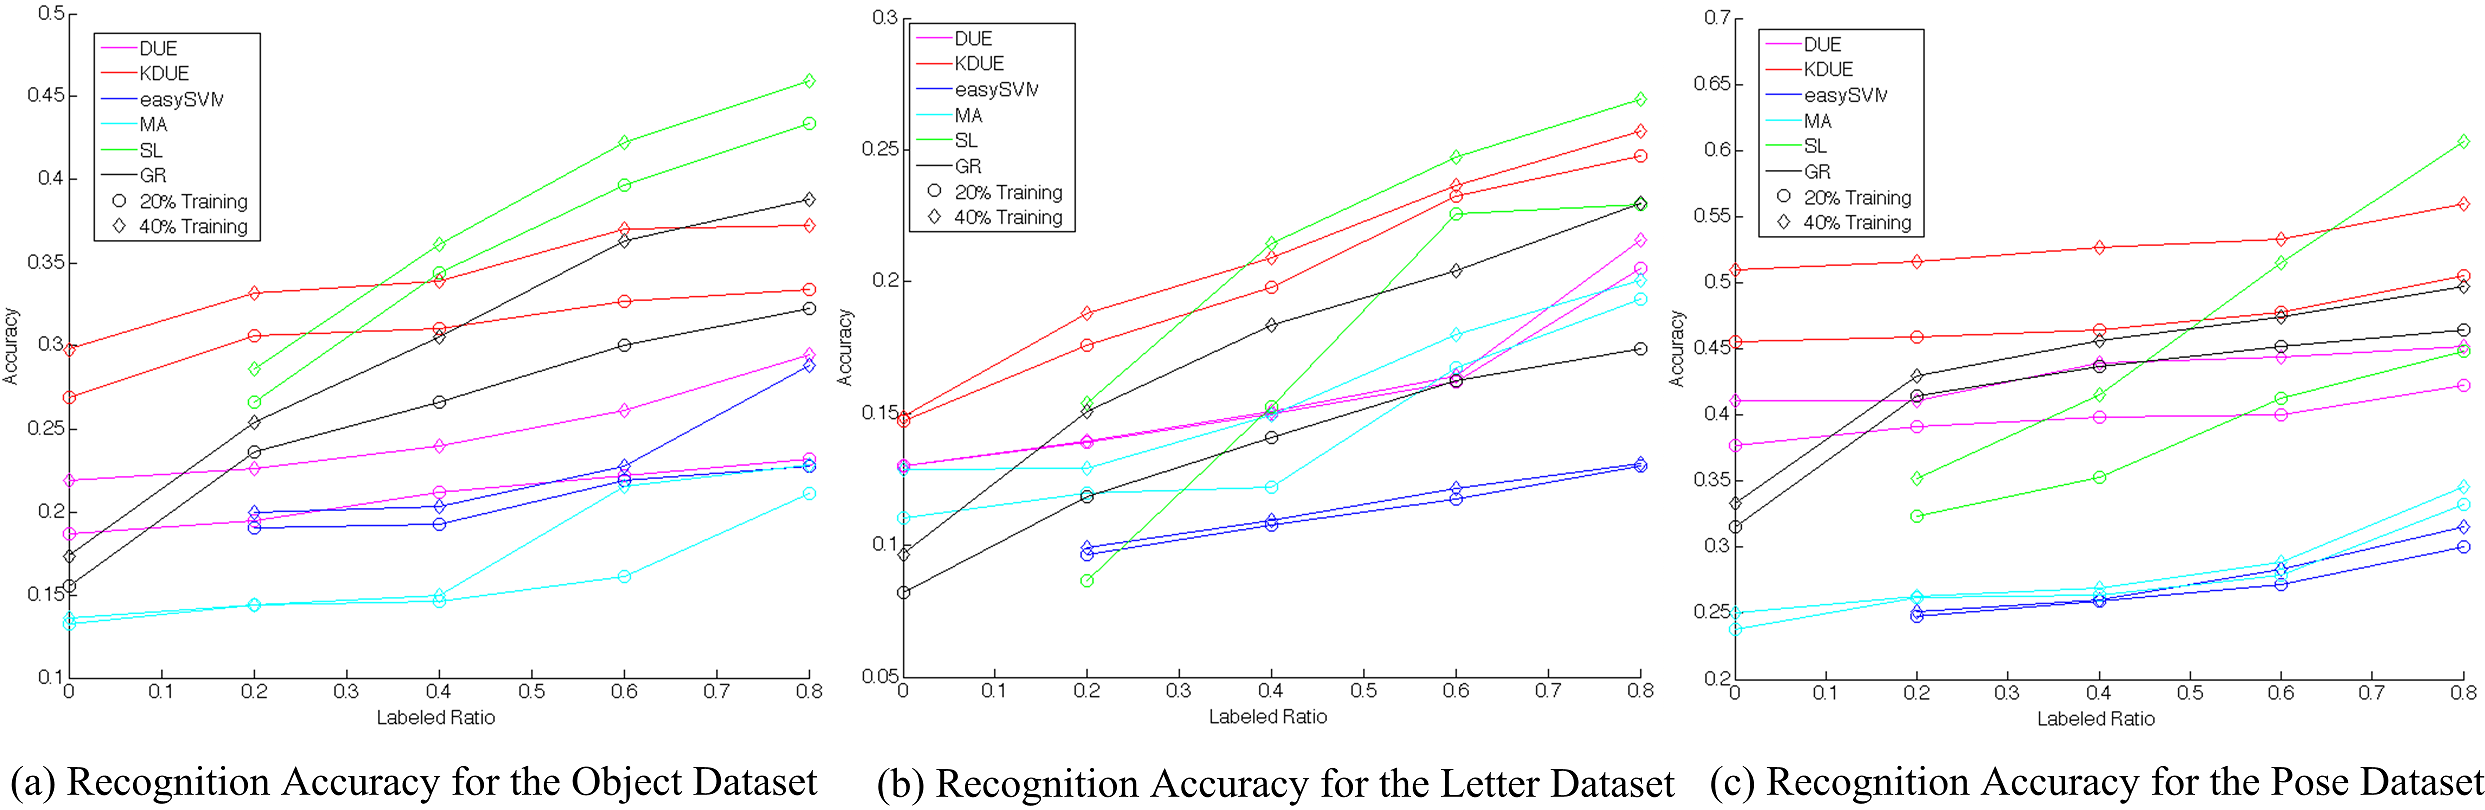
\includegraphics[scale=1.6]{stat_new_2.png}
\end{center}
\caption{Cross-domain recognition accuracy comparisons.(Best viewed in color)}
\label{stat_2}
\end{figure*}

The capabilities of the baselines and our approach are summarized in Table \ref{compare}. SL learns similarities between pairs of samples across domains to maximize the discrimination among categories in these domains, and it does not allow more than two source domains. While the similarity learning strategy can account for unlabeled correspondences in principle, SL does not explicitly do so. To apply SL in the presence of multiple source domains, we regard the multiple source domains as a single domain, use the minimum dimension among them as the dimension for this single domain, and reduce all higher-dimensional source features to this minimum dimension by a dimension-reducing operator that is appropriate for each dataset (to be discussed shortly).  Classification is realized by the nearest neighbor rule. GR is a feature augmentation method that interpolates feature subspaces from the source(s) to the target, and it requires the same dimension for all sources.  To utilize heterogenous features from the source domains, we again determine the minimum dimension among all sources, and reduce higher-dimensional source features to the minimum dimension by appropriate dimensionality reduction. We implement both \cite{Gopalan:Grassmann} (with Partial Least Squares as the classifier) and \cite{Gong:Grassmann} (with nearest neighbor as the classifier) and report the best performance between the two. MA seeks a linear dimension reducing transform to align the source and target domains such that the sample topology is preserved while maximizing discrimination. It does not adaptively weight different domains, and can therefore be regarded as a special case of our approach. We use a separate one-against-one multi-class SVM in the latent domain as the classifier for MA, as well as for DUE and KDUE. EasySVM builds cross-domain feature vectors by replicating feature vectors from different domains and requires the same dimension for all domains. To apply easySVM in the presence of heterogeneity and unlabeled correspondences, we create a modification of CCA as follows. Let $\mathbf{C}_{i,j}$ be the sample correlation matrix between domain $i$ and domain $j$ ($i,j=1,2,\cdots,V$) computed from pair-wise correspondences. Our modified CCA finds linear transformations $\mathbf{w}_{i}, i=1,2,\cdots,V$ (from the original domains to the shared $k$-dimensional domain) as
\begin{equation}
\label{multiCCA}
\max_{\mathbf{w}_{i}}\sum_{i,j=1,i\ne j}^{V}tr(\mathbf{w}_{i}^{T}\mathbf{C}_{i,j}\mathbf{w}_{j}),  \textup{s.t.}\hspace{3pt}\sum_{i=1}^{V}tr(\mathbf{w}_{i}^{T}\mathbf{C}_{i,i}\mathbf{w}_{i})=kV,
\end{equation}
which is also solved by a generalized eigen decomposition. We feed the outputs from this modified CCA into easySVM, and use this two-step procedure as a whole.



\noindent\textbf{Protocol}. Even though DUE and KDUE (as well as MA and easySVM) do not make formal distinctions between the source domain(s) and the target domain but can uniformly leverage all information from all domains, we follow the protocol of \cite{Saenko:ML,Kulis:ML,Gopalan:Grassmann} in specifying a target domain. Specifically, in each trial we select one domain as the target domain, and use all others as sources. We use for training all available source samples, along with varying numbers (20\%, 40\%) of the samples available in the target domain. The left-out samples in the target domain are used for testing. The training samples are further divided into two sets: labelled ones, and unlabeled correspondences. This means a training sample is used as either an isolated labeled one, or an unlabeled one with its correspondence in another domain. We vary the ratio of labeled samples among all training samples in the target domain through 0\%,20\%, 40\%, 60\%, and 80\%, where 0\% means all training samples in the target domain are unlabeled, with some or all of them having correspondences in the source domain(s)\footnote{Labeled correspondences can be exploited either for their labels or for their correspondences and thus are trivial cases. Though DUE/KDUE handles all conditions seamlessly, we set the correspondences unlabeled to make the condition non-trivial and match the scenario described in the introduction.}.


\begin{figure}
\begin{center}
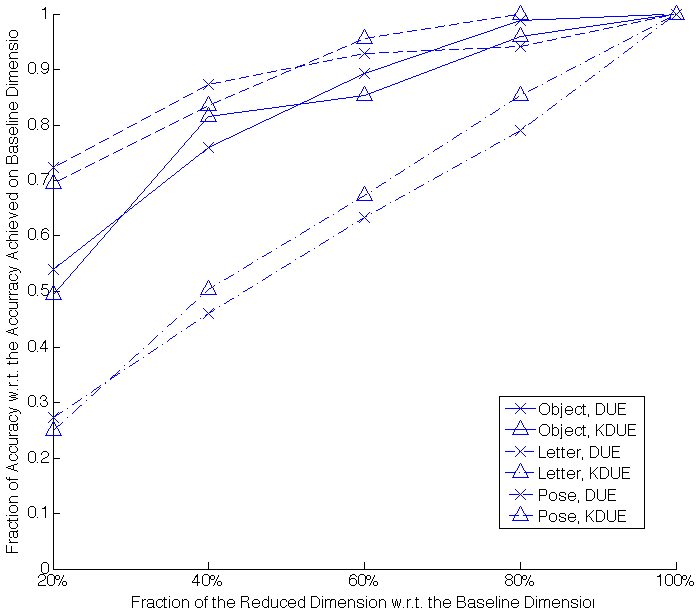
\includegraphics[scale=0.25]{sensi_new.png}
\end{center}
\caption{Sensitivities to the variation of the latent common domain dimension.}
\label{sensi}
\end{figure}



%This data partitioning scheme is always applicable to DUE and KDUE regardless of dataset and regardless of the available amounts or formats of the annotation. It is also straightforward for all baselines on the facial pose dataset where all samples have cross-domain correspondences by construction: The unlabeled correspondences are used in SL and GR to compute CCA for dimension reduction, and in easySVM to compute the modified CCA.  For the object dataset correspondences only exist between DSLR and webcam domains, so when either of these two is serving as target we can use the correspondences to compute CCA for SL and GR (we applying the same CCA transform to the Amazon domain and simply aggregate the samples from the two sources). When the Amazon domain serves as the target, no correspondence exists between the target and sources. In this case, we first compute CCA between the two sources using unlabeled correspondence and merge them, and then approximate the unlabeled correspondences between the merged source and the target by the pairs of samples of the same category (we call this approximation category-based correspondence), and compute CCA between the merged source and the target. A similar issue exists on this dataset for easySVM, which requires correspondences among all involved domains. We again use category-based correspondence to approximate the unlabeled correspondences for easySVM. However, note that the object dataset has the same dimension for all domains, which means that alternatively we can trivially merge two source domains without applying any dimension-reducing transform.\footnote{We tried both strategies and report the best performance.} For the letter dataset, the approximation of category-based correspondence is used for CCA for dimension reduction whenever necessary.

This data partitioning scheme is always applicable to DUE and KDUE regardless of dataset and regardless of the available amounts or formats of the annotation. It is also straightforward for all baselines on the facial pose dataset where all samples have cross-domain correspondences by construction. For the letter dataset and the object dataset's Amazon domain, we simulate unlabeled correspondences by all pairs of samples of the same category. We call this approximation category-based correspondence. For the methods that do not support heterogeneous domains (GR and easySVM, see Table~\ref{compare}), or require one  single-dimensional source (SL), unlabeled correspondences (real or simulated) are used to compute CCA (modified CCA for easySVM) and use it to reduce features to the same dimension, as necessary.

\begin{figure}
\begin{center}
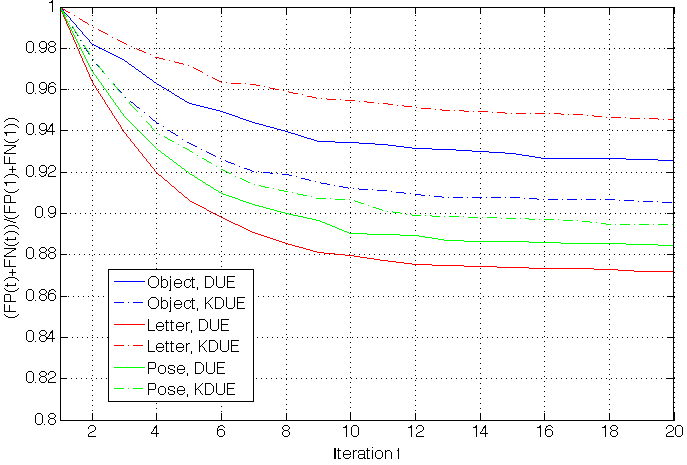
\includegraphics[scale=0.25]{conv.png}
\end{center}
\caption{The average convergence curve of the combined false positive rate (FP) and false negative rate (FN) w.r.t. the initial combined rate.}
\label{conv}
\end{figure}


\noindent\textbf{Results}. We perform five independent runs for each combination of target domain and training/labeling ratios, and report the average cross-domain recognition accuracies in Figure \ref{stat_2}. The dimension of the latent common domain $k$ is fixed to be half of the minimum dimensions of all involved domains for DUE and KDUE. Note that when no labeled samples in the target domain are available, neither SL nor easySVM can operate. On the object dataset (Figure \ref{stat_2}(a)), SL demonstrates the highest recognition performance, while KDUE and GR comparably follow SL given a sufficient portion of labeled target samples. When the number of labeled target samples drops to zero, KDUE performs better than GR, due to the fact that GR does not fully consider instance correspondences. There exist no significant differences among the other baselines when labels are abundant in the target domain, but DUE stands out when the target domain is completely unlabeled. When the source and the target are heterogeneous as is the case in the letter dataset (Figure \ref{stat_2}(b)), MA, DUE, and KDUE show superiority, with KDUE slightly standing out. SL is successful in learning cross-domain similarities with sufficient labeled training samples available in the target domain, and its performance degrades to that of the embedding-based methods when the number of labels decreases. An important message conveyed from this experiment is that the heterogeneity among domains substantially undermines the strategy of integrating an ad-hoc dimension reduction into a homogeneous domain adaptation algorithm. The facial pose dataset (Figure \ref{stat_2}(c)) represents a cross-domain problem with the full range of challenges, on which KDUE succeeds over all when provided fewer labels on fewer target training samples but is outperformed by SL given more labeled training samples. Meanwhile, DUE compares to the method of GR, which aims to establish an explicit cross-domain feature representation. One salient observation, is that KDUE demonstrates strength especially when the target domain is weakly annotated.


\begin{figure*}[t]
\begin{center}
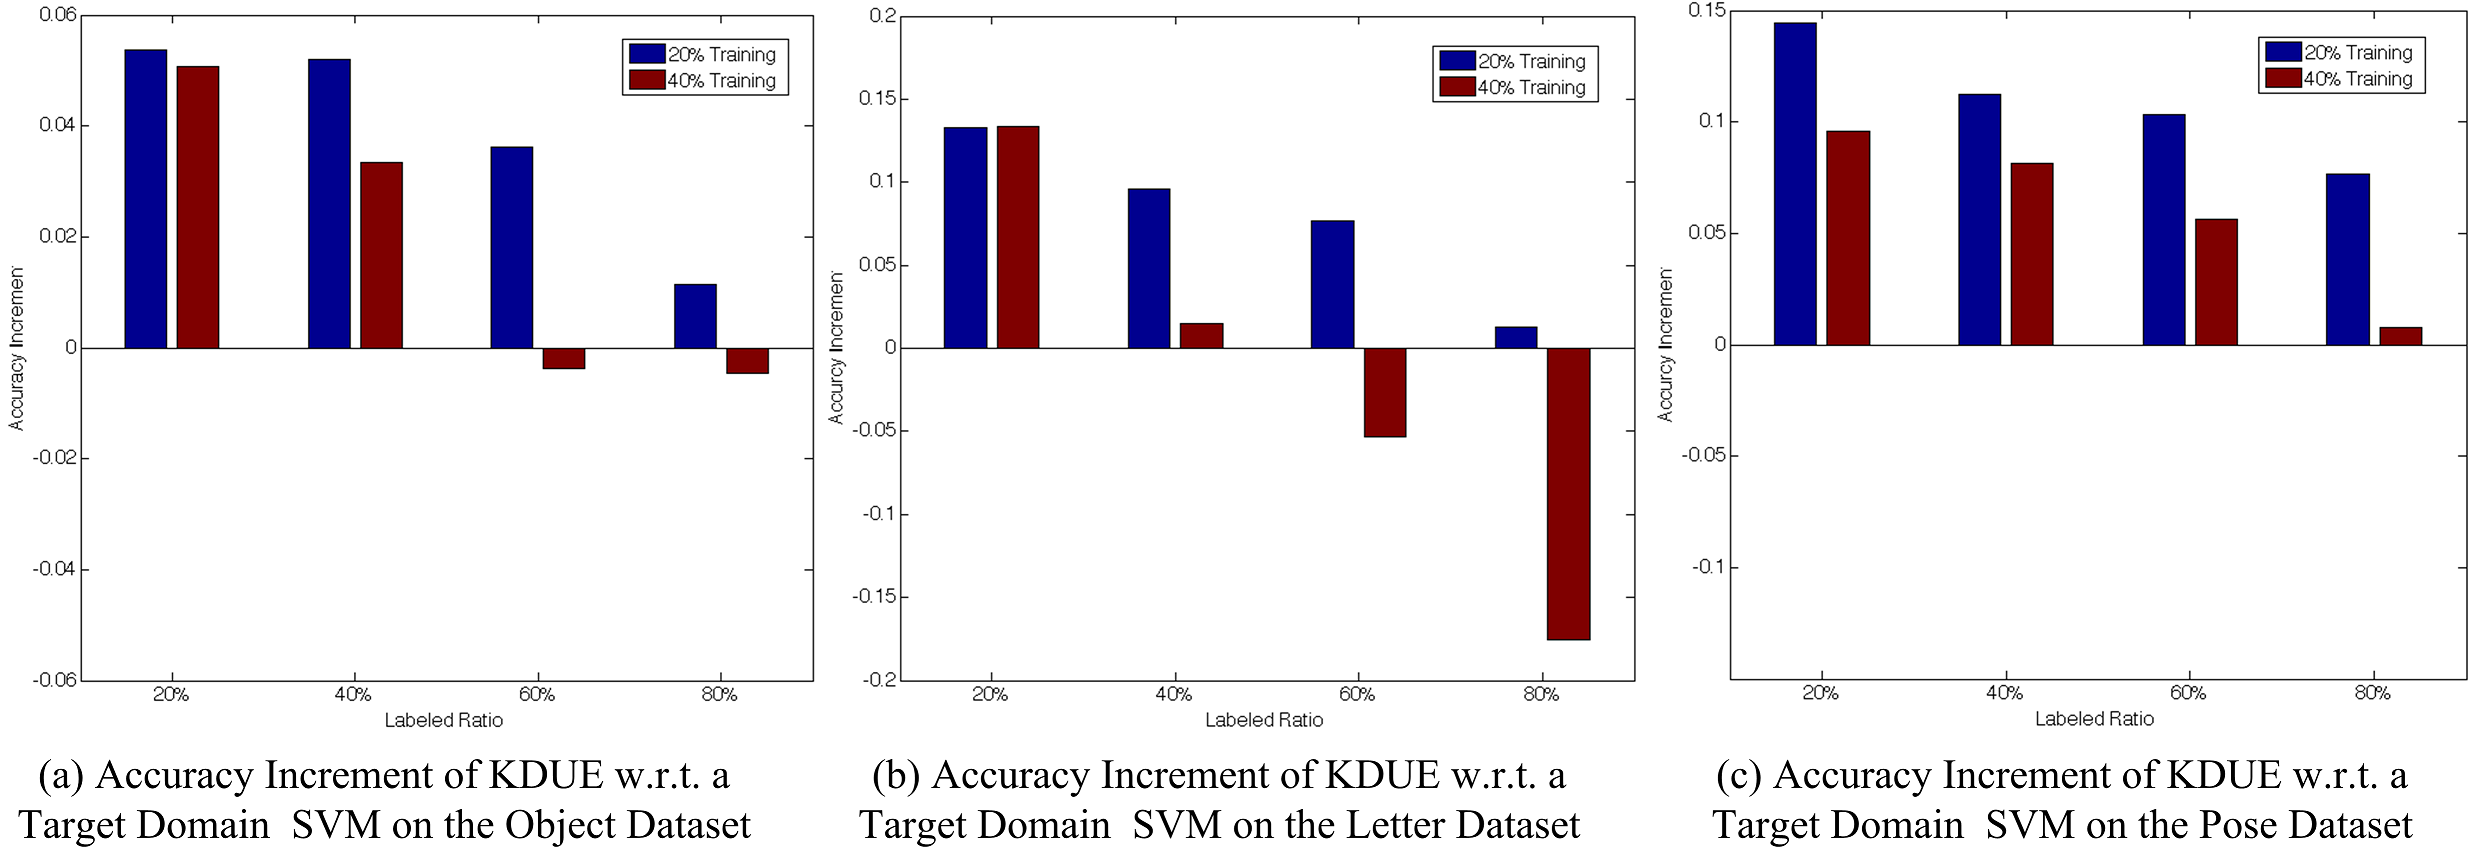
\includegraphics[scale=1.6]{stat_new_1.png}
\end{center}
\caption{The accuracy increment with respect to a baseline SVM trained in the target domain.}
\label{stat_1}
\end{figure*}


The dimension of the latent common domain $k$ in DUE or KDUE is a major factor effecting the embedding. We reduce the dimension to 80\%, 60\%, 40\%, and 20\% to evaluate the sensitivity of the performance. As Figure \ref{sensi}, shows, recognition accuracies drop moderately for object and face pose datasets, but drastically decrease on the letter dataset, again highlighting the challenge of heterogeneous domains.

The overall algorithm alternating between solving for the embedding transform and solving for the domain-specific penalties represents a greedy search and its convergence is not theoretically guaranteed. To check the empirical convergence performance, we plot the average combined false positive rate and false negative rate as a function of iteration $h$, relative to the initial combined error rate at $h=1$, in Figure \ref{conv}. It turns out that the combined error rate decreases on average.   It is also evident that the final false positive and false negative rate is reduced by 6\%-13\% when the adaptive penalization is enabled.

Finally, we investigate how much transferring source domain knowledge actually helps the recognition in the target domain. For this purpose, we train a one-against-one multi-class SVM in the target domain using the labeled training samples in the target domain, and then classify the testing samples. We show the accuracy increments of KDUE with respect to this baseline SVM in Figure \ref{stat_1}: Positive increments occur when fewer training and fewer labeling are available in the target, which is exactly the typical scenario for the application of domain transfer.



\noindent\textbf{Conclusion}. In summary, KDUE is competitive with the baselines, and outperforms them in the presence of heterogeneous domains and limited target labeling. The linear version, DUE, is generally comparable to the state-of-art. Both DUE and KDUE allow the maximal flexibility in encoding various generalizations of the domain adaptation problem. Their main distinction is their performance in conditions of multiple heterogeneous domains with fewer target labels but abundant unlabeled correspondences among some or all of the domains.

Another potential benefit of the proposed approaches, due to their operation on feature spaces instead of SVM parameters, is their suitability for transferring new categories, \textit{i.e.}, the test data belongs to categories for which we have labels only in the source domain(s), a property shared by SL,GR, and MA as well. An empirical study of their performance on transferring new categories will be worthwhile in the future.

{\footnotesize 
\bibliographystyle{ieee}
\bibliography{duebib}
}




\end{document}
